\documentclass[11pt,a4paper]{article}

\usepackage[utf8]{inputenc}
\usepackage[T1]{fontenc}
\usepackage[spanish,es-tabla]{babel}
\usepackage[margin=2.4cm]{geometry}
\usepackage{graphicx}
\usepackage{float}
\usepackage{booktabs}
\usepackage{array}
\usepackage{amsmath}
\usepackage{caption}
\usepackage{enumitem}
\usepackage{longtable}
\usepackage{xcolor}
\usepackage[hidelinks]{hyperref}

\captionsetup{font=small,labelfont=bf}
\setlength{\parskip}{0.5em}
\setlength{\parindent}{0pt}
\renewcommand{\arraystretch}{1.15}

\title{\vspace{-1.5cm}\textbf{Laboratorio 6: An\'alisis de redes sociales en YouTube}}
\author{Grupo \#7 \\[2pt]
Marco Carbajal (23025) \quad Carlos Angel (23010) \quad Diego Monroy (23318)\\[4pt]
\small Universidad del Valle de Guatemala --- Facultad de Ingenier\'ia\\
\small CC3084 Data Science --- Secci\'on 20 --- Semestre II, 2026}
\date{6 de septiembre de 2026}

\begin{document}
\maketitle

\begin{abstract}
\noindent Se analizan dos conjuntos de datos de YouTube (\texttt{youtube\_videos.csv}, 293 videos;
\texttt{youtube\_comments.csv}, 406 comentarios) para estudiar la estructura de participaci\'on de los
usuarios, la relaci\'on entre canales y temas, y el contenido de las conversaciones. Se documenta la
carga e integraci\'on de los datos, el diagn\'ostico de calidad y la limpieza de texto, un an\'alisis
exploratorio, la construcci\'on de una red bipartita autor--video con sus dos proyecciones, el an\'alisis
de topolog\'ia y fragmentaci\'on, la detecci\'on de comunidades con Louvain, el c\'alculo de centralidades
y puntos de articulaci\'on, y un an\'alisis de sentimiento basado en un l\'exico de polaridad en espa\~nol
adaptado al dominio. El hallazgo transversal es que la participaci\'on observada est\'a fuertemente
concentrada en pocos videos y canales pero repartida entre muchos autores que aparecen una sola vez,
de modo que la red tiene forma de estrellas d\'ebilmente unidas por menos de diez autores puente. Todas
las conclusiones est\'an limitadas por el procedimiento de recolecci\'on: el 93.5\,\% de los videos del
cat\'alogo no tiene comentarios recolectados.
\end{abstract}

\tableofcontents
\bigskip
\hrule

\section{Carga, comprensi\'on e integraci\'on de los datos}

\subsection{Carga de los archivos}
Se cargaron \texttt{youtube\_videos.csv} (293 filas, 20 variables) y \texttt{youtube\_comments.csv}
(406 filas, 17 variables) con \texttt{pandas}. No hay filas ni llaves duplicadas en ninguno de los dos
archivos.

\subsection{Unidad de observaci\'on, llave primaria y variables relevantes}
En \texttt{youtube\_videos.csv} la unidad de observaci\'on es el \textbf{video} y la llave primaria es
\texttt{video\_id} (sin duplicados en 293 filas). Variables relevantes: \texttt{channel\_id}
(identificador estable del canal), \texttt{title} y \texttt{description} para an\'alisis tem\'atico,
\texttt{view\_count} para popularidad, \texttt{category}, \texttt{source\_query} y \texttt{source\_group}
para reconstruir el muestreo, y \texttt{publish\_date} como \'unica marca temporal absoluta.

En \texttt{youtube\_comments.csv} la unidad de observaci\'on es el \textbf{comentario} y la llave primaria
es \texttt{comment\_id} (sin duplicados en 406 filas). Variables relevantes: \texttt{video\_id} como
llave for\'anea, \texttt{author\_channel\_id} para identificar al autor, \texttt{text} para el contenido,
\texttt{like\_count\_text} y \texttt{reply\_count} como medidas de recepci\'on, y \texttt{channel\_id},
que identifica al canal due\~no del video comentado, no al autor.

\subsection{Relaci\'on entre canal, video, autor, comentario, categor\'ia y consulta}
La estructura es jer\'arquica en dos niveles. Un canal (\texttt{channel\_id}) publica varios videos:
97 canales para 293 videos, con mediana de 1 video por canal y m\'aximo de 32. Cada video puede recibir
varios comentarios y cada comentario tiene un autor (\texttt{author\_channel\_id}), un identificador de
cuenta distinto del canal que public\'o el video. La \textbf{categor\'ia} es un atributo del video
asignado por YouTube; se hereda al unir las tablas pero no describe al comentario ni al autor. La
\textbf{consulta de b\'usqueda} es un atributo del procedimiento de recolecci\'on: \texttt{source\_query}
describe c\'omo se encontr\'o el registro y \texttt{source\_group} clasifica la estrategia. Ninguna
describe el tema del video de forma confiable, por lo que se usan para auditar cobertura, no como
variable tem\'atica. Adem\'as, autores de comentarios y canales de video son conjuntos \textbf{disjuntos}:
ninguno de los 332 \texttt{author\_channel\_id} aparece como \texttt{channel\_id} de un video.

\subsection{Integraci\'on por \texttt{video\_id}}
Los \textbf{406 comentarios} (100\,\%) se asociaron con un video, as\'i que no hay comentarios hu\'erfanos.
La relaci\'on es fuertemente asim\'etrica en el otro sentido: solo \textbf{19 de 293 videos (6.5\,\%)} y
\textbf{8 de 97 canales} tienen comentarios recolectados. Las columnas redundantes coinciden al 100\,\%
para \texttt{channel\_id}, \texttt{channel\_name} y el t\'itulo, lo que confirma que la uni\'on es
consistente. La excepci\'on es \texttt{source\_group}, que coincide en apenas 53.7\,\% de los casos
porque el mismo video fue alcanzado por una estrategia distinta en cada archivo.

\section{Calidad, limpieza y preprocesamiento}

\subsection{Diagn\'ostico inicial de calidad}
\begin{table}[H]
\centering
\caption{S\'intesis del diagn\'ostico de calidad.}
\begin{tabular}{p{4.3cm} p{10.5cm}}
\toprule
\textbf{Dimensi\'on} & \textbf{Hallazgo} \\
\midrule
Dimensiones & videos $293\times20$; comentarios $406\times17$. \\
Duplicados & 0 filas y 0 llaves duplicadas en ambos archivos. \\
Faltantes (videos) & \texttt{published\_time} y \texttt{view\_count\_text}: 13 (4.4\,\%);
  \texttt{description\_snippet}: 25 (8.5\,\%); \texttt{description}: 26 (8.9\,\%). \\
Faltantes (comentarios) & 0 nulos declarados, pero \texttt{like\_count\_text} guarda
  \textbf{189 cadenas en blanco (46.6\,\%)} que el conteo de nulos no detecta. \\
Variables constantes & \texttt{is\_pinned} (\texttt{False}) y \texttt{viewer\_rating} (vac\'ia)
  en comentarios; se descartan. \\
Consistencia IDs/nombres/handles & relaci\'on \textbf{uno a uno} para canales y autores;
  \texttt{video\_id} de 11 caracteres, IDs de canal con patr\'on \texttt{UC}+22, handles con
  prefijo \texttt{/@}. \texttt{owner\_handle} $\equiv$ \texttt{channel\_handle} y
  \texttt{upload\_date} $\equiv$ \texttt{publish\_date}. \\
At\'ipicos & \texttt{view\_count} muy asim\'etrica: mediana 1\,175, l\'imite intercuart\'ilico
  18\,340, \textbf{49 videos} por encima, encabezados por un video de Luisito Comunica con
  8.19 millones. No son errores; se conservan y se usa escala logar\'itmica. \\
\bottomrule
\end{tabular}
\end{table}

\textbf{Hallazgo relevante para la interpretaci\'on:} 36 de las 406 filas (8.9\,\%) tienen un
\texttt{comment\_id} con sufijo de respuesta y su comentario padre est\'a en el mismo archivo, de modo
que la afirmaci\'on de que ``cada fila es un comentario principal'' no se cumple del todo. Adem\'as, la
suma de \texttt{reply\_count} es 51 mientras que solo hay 36 respuestas presentes: la cobertura de
segundo nivel es incompleta.

\subsection{Variables que no pueden usarse o requieren precauci\'on}
\begin{longtable}{l l l p{6.6cm}}
\toprule
\textbf{Variable} & \textbf{Archivo} & \textbf{Decisi\'on} & \textbf{Raz\'on} \\
\midrule
\endhead
\texttt{viewer\_rating} & comentarios & descartar & vac\'ia en las 406 filas \\
\texttt{is\_pinned} & comentarios & descartar & constante \texttt{False} \\
\texttt{owner\_handle} & videos & descartar & copia exacta de \texttt{channel\_handle} \\
\texttt{upload\_date} & videos & descartar & copia exacta de \texttt{publish\_date} \\
\texttt{video\_title} & comentarios & descartar & redundante con la uni\'on por \texttt{video\_id} \\
\texttt{published\_time} & videos & precauci\'on & fecha relativa al momento de recolecci\'on \\
\texttt{published\_text} & comentarios & precauci\'on & fecha relativa; no permite ordenar con exactitud \\
\texttt{view\_count\_text} & videos & precauci\'on & texto con separador de miles y 13 faltantes \\
\texttt{like\_count\_text} & comentarios & precauci\'on & 189 blancos que se interpretan como cero \\
\texttt{reply\_count} & comentarios & precauci\'on & no identifica autores; \textbf{no genera aristas} \\
\texttt{channel\_name} & ambos & precauci\'on & etiqueta visible, no identificador \\
\texttt{source\_query} & ambos & precauci\'on & describe el muestreo, no el tema \\
\texttt{source\_group} & ambos & precauci\'on & difiere entre tablas para el mismo video \\
\texttt{keywords} & videos & precauci\'on & lista vac\'ia en 162 de 293 videos \\
\bottomrule
\end{longtable}

\texttt{reply\_count} es la variable m\'as delicada: el enunciado advierte que no identifica a los
autores de las respuestas y que no debe leerse como arista entre usuarios. Se usa \'unicamente como
atributo de recepci\'on del comentario.

\subsection{Normalizaci\'on de identificadores y nombres}
Se garantiz\'o que las llaves (\texttt{video\_id}, \texttt{channel\_id}, \texttt{comment\_id},
\texttt{author\_channel\_id}) sean cadenas sin espacios y se mantengan como identificadores en todas
las tablas derivadas. Los nombres visibles y los handles se conservan en columnas separadas, solo como
etiquetas para las visualizaciones. Como la relaci\'on identificador--nombre--handle es uno a uno, no
hay ambig\"uedad que resolver; los recortes y la verificaci\'on de formato se aplican de todos modos
para que el procedimiento sea reproducible.

\subsection{Conversi\'on de variables de conteo almacenadas como texto}
\texttt{like\_count\_text} no contiene abreviaturas ni separadores de miles: valores enteros simples
o cadenas en blanco. Las \textbf{189 cadenas en blanco se imputan a cero} porque YouTube omite el
contador cuando un comentario no tiene reacciones y el cero no aparece expl\'icito en ninguna fila.
Es una decisi\'on de interpretaci\'on, no un dato observado, y afecta al 46.6\,\% de los comentarios.
\texttt{view\_count\_text} s\'i trae separador de miles y el sufijo ``vistas''; se parse\'o solo para
auditor\'ia: coincide con \texttt{view\_count} en 227 de 280 registros con dato y en el resto la
diferencia mediana es 0.05\,\%. Para todos los c\'alculos se usa \texttt{view\_count}.

\subsection{Versiones del texto}
Se conservan dos columnas. \texttt{texto\_original} es una copia sin modificar de \texttt{text} y sirve
para auditor\'ia y para el an\'alisis de sentimiento, porque este depende de negaciones, may\'usculas
sostenidas, signos de exclamaci\'on y emojis que la limpieza elimina. \texttt{texto\_limpio} es la
versi\'on normalizada y lematizada que se usa para frecuencias de palabras y bigramas.

\subsection{Decisiones de limpieza aplicadas a \texttt{texto\_limpio}}
\begin{itemize}[leftmargin=1.4em,itemsep=1pt]
  \item \textbf{Min\'usculas:} para unificar ``Guatemala''/``guatemala''; se pierde el \'enfasis por
        may\'usculas sostenidas, raz\'on adicional para conservar el texto original.
  \item \textbf{URL:} se eliminan (no aportan vocabulario); solo 1 comentario tiene enlace.
  \item \textbf{Hashtags y menciones:} se separa el s\'imbolo y se conserva la palabra; solo hay
        1 hashtag y 5 menciones en todo el corpus, guardados adem\'as en columnas propias.
  \item \textbf{Puntuaci\'on y n\'umeros:} se eliminan; los n\'umeros son montos y a\~nos demasiado
        heterog\'eneos para tratarlos como categor\'ia.
  \item \textbf{Stopwords:} lista en espa\~nol de NLTK (313 t\'erminos) y descarte de tokens de
        $\leq 2$ caracteres.
  \item \textbf{Lematizaci\'on:} spaCy \texttt{es\_core\_news\_sm} con los componentes de parseo y
        entidades desactivados. Introduce algo de ruido en palabras sin tilde, pero el saldo favorece
        el conteo de frecuencias.
  \item \textbf{Emojis:} se eliminan de \texttt{texto\_limpio} pero se cuentan antes: 61 comentarios
        contienen al menos uno, 199 en total, y 5 comentarios son solo emojis.
\end{itemize}

\subsection{Efecto cuantificado de la limpieza}
\begin{table}[H]
\centering
\caption{Efecto de la limpieza sobre los 406 comentarios.}
\begin{tabular}{l r}
\toprule
M\'etrica & Valor \\
\midrule
Registros eliminados & 0 \\
Textos modificados & 396 de 406 \\
Tokens antes / despu\'es & 9\,769 / 5\,103 ($-47.8\,\%$) \\
Vocabulario antes / despu\'es & 3\,171 / 2\,019 \\
Textos vac\'ios antes / despu\'es & 0 / 5 \\
Duplicados exactos antes / despu\'es & 2 / 6 \\
\bottomrule
\end{tabular}
\end{table}
No se elimina ning\'un registro. Cinco comentarios quedan vac\'ios porque eran solo emojis o una
palabra corta (``que?''); se conservan porque siguen contando como participaci\'on v\'alida para la
red, pero quedan fuera del an\'alisis de frecuencias. Los duplicados pasan de 2 a 6: los 2 originales
son casos reales (mismo autor, mismo texto, mismo video, \texttt{comment\_id} distinto) y los 4
adicionales aparecen porque la normalizaci\'on colapsa variantes como ``Excelente.''/``EXCELENTE''.
Ninguno se elimina.

\section{An\'alisis exploratorio}

\subsection{Descripci\'on de los elementos m\'inimos}
\begin{table}[H]
\centering
\caption{Conteos generales.}
\begin{tabular}{l r l r}
\toprule
Elemento & Valor & Elemento & Valor \\
\midrule
Videos (cat\'alogo) & 293 & Videos con $\geq 1$ comentario & 19 \\
Canales (cat\'alogo) & 97 & Canales con $\geq 1$ comentario & 8 \\
Comentarios & 406 & Categor\'ias de video & 11 \\
Autores \'unicos & 332 & Consultas (videos / comentarios) & 21 / 6 \\
\bottomrule
\end{tabular}
\end{table}

\textbf{Videos por canal:} media 3.02, mediana 1, m\'aximo 32; 65 de 97 canales (67\,\%) aportan un
solo video. Los canales m\'as presentes en el cat\'alogo son Gobierno de la Rep\'ublica (32),
Municipalidad de Guatemala (27), Quorum (18) y PrensaLibre (17).

\textbf{Comentarios y autores por video} (Tabla~\ref{tab:porvideo}): la raz\'on autores/comentarios va
de 0.71 a 1.0, es decir que casi todos los comentarios provienen de personas distintas.

\begin{table}[H]
\centering
\caption{Videos con comentarios recolectados, ordenados por n\'umero de comentarios.}
\label{tab:porvideo}
\small
\begin{tabular}{l l r r r r r}
\toprule
Video & Canal & Coment. & Autores & Likes & Resp. & Vistas \\
\midrule
Qu\'e rico come tu diputado & Quorum & 161 & 128 & 358 & -- & 11\,775 \\
La cooptaci\'on de W. Mazariegos en la USAC & Quorum & 50 & 49 & 91 & -- & 10\,156 \\
Inician trabajos del Puente Belice II & Gobierno & 45 & 32 & 90 & -- & 11\,670 \\
Plan 2032 Ciudad de Guatemala & Municipalidad & 25 & 25 & 1\,697 & -- & 304\,089 \\
Conferencia de Prensa del Gobierno & Gobierno & 25 & 19 & 20 & -- & 3\,628 \\
EE.UU. env\'ia a mexicanos deportados & N. Telemundo & 25 & 18 & 25 & -- & 14\,200 \\
Arroz con pollo a la MONOPOLIO & Quorum & 16 & 16 & -- & -- & 1\,954 \\
Capturan a presuntos delincuentes\dots & Noti7 & 14 & 13 & -- & -- & -- \\
Internet: escoger el menos malo & Quorum & 12 & 10 & -- & -- & 717 \\
\midrule
\multicolumn{2}{l}{\emph{otros 10 videos}} & $\leq 7$ & $\leq 7$ & & & \\
\bottomrule
\end{tabular}
\end{table}

\textbf{Visualizaciones (293 videos):} mediana 1\,175, media 60\,430, m\'aximo 8.19\,M.
\textbf{Me gusta por comentario:} mediana 1, media 5.73, 189 comentarios con 0.
\textbf{Respuestas:} 30 comentarios con \texttt{reply\_count} $>0$, suma 51, m\'aximo 7.

\textbf{Categor\'ias:} News \& Politics domina con 138 videos y 335 comentarios. People \& Blogs tiene
66 videos y \textbf{cero} comentarios recolectados, lo que confirma que la cobertura depende del
muestreo y no del tema.

\textbf{Consultas:} 21 distintas para videos frente a 6 para comentarios; \texttt{@quorumgt/videos}
sola aporta 231 de 406 comentarios. Por estrategia de recolecci\'on: \texttt{topic} 363 comentarios
(12 videos), \texttt{channel} 43 (7 videos), \texttt{official\_gov} \textbf{0} (105 videos).

\textbf{Hashtags y menciones:} 1 y 5 respectivamente en todo el corpus.
\textbf{Vocabulario limpio:} 2\,019 t\'erminos sobre 5\,103 tokens. Palabras m\'as frecuentes tras la
lematizaci\'on: verbos auxiliares y luego \emph{pueblo, guatemala, diputado, pagar, dinero}. Bigramas:
\emph{presidente bernardo, bernardo arevalo, pacto corrupto, diputado ser} --- eje pol\'itico claro
(Figura~\ref{fig:palabras}).

\subsection{Concentraci\'on de la participaci\'on}
Un solo video, ``Qu\'e rico come tu diputado'', re\'une el \textbf{39.7\,\%} de los comentarios; los
tres primeros acumulan 63.1\,\% y los cinco primeros 75.4\,\%. El \'indice de Gini sobre los 19 videos
comentados es \textbf{0.66}, y sube a \textbf{0.978} sobre los 293 videos del cat\'alogo (274 con cero
comentarios). A nivel de canal, Quorum aporta 256 comentarios (63.1\,\%) y los tres canales principales
suman 86.5\,\%. Del lado de los autores el patr\'on se invierte: \textbf{286 de 332 (86.1\,\%)}
escribieron un \'unico comentario y solo 9 participaron en m\'as de un video. Esa combinaci\'on
anticipa la forma de estrella de la red bipartita (Figura~\ref{fig:concentracion}).

\subsection{Popularidad frente a participaci\'on}
Entre los 19 videos comentados la asociaci\'on es fuerte y positiva: Spearman \textbf{0.811}
($p<0.001$, $n=19$) y correlaci\'on 0.718 entre los logaritmos. No es proporcional: la tasa de
comentarios por mil vistas var\'ia en m\'as de dos \'ordenes de magnitud, desde 19.2 (video con 52
vistas) hasta 0.08 en ``Plan 2032 Ciudad de Guatemala'' (304\,089 vistas, 25 comentarios). Adem\'as,
la mediana de vistas de los videos comentados (1\,954) es apenas superior a la de los no comentados
(1\,150): la selecci\'on de videos para recolectar comentarios no sigui\'o el criterio de popularidad.
\textbf{Limitaciones de ambos conteos:} \texttt{view\_count} es un acumulado desde la publicaci\'on,
mientras que el n\'umero de comentarios recolectados es un tope impuesto por el \emph{scraping}, no el
n\'umero real de comentarios del video.

\subsection{Visualizaciones}
\begin{figure}[H]
\centering
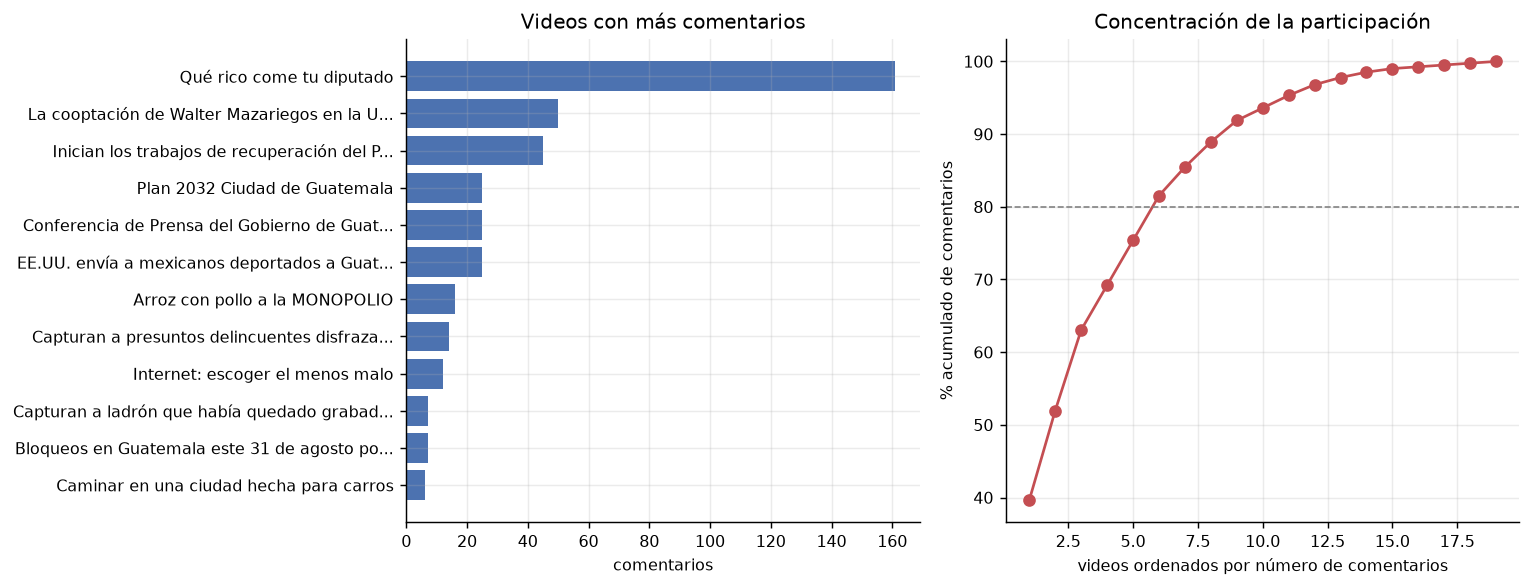
\includegraphics[width=\linewidth]{figuras/eda_concentracion.png}
\caption{Videos con m\'as comentarios (izq.) y curva de concentraci\'on acumulada (der.): el 80\,\% de
los comentarios se alcanza en el sexto de diecinueve videos.}
\label{fig:concentracion}
\end{figure}

\begin{figure}[H]
\centering
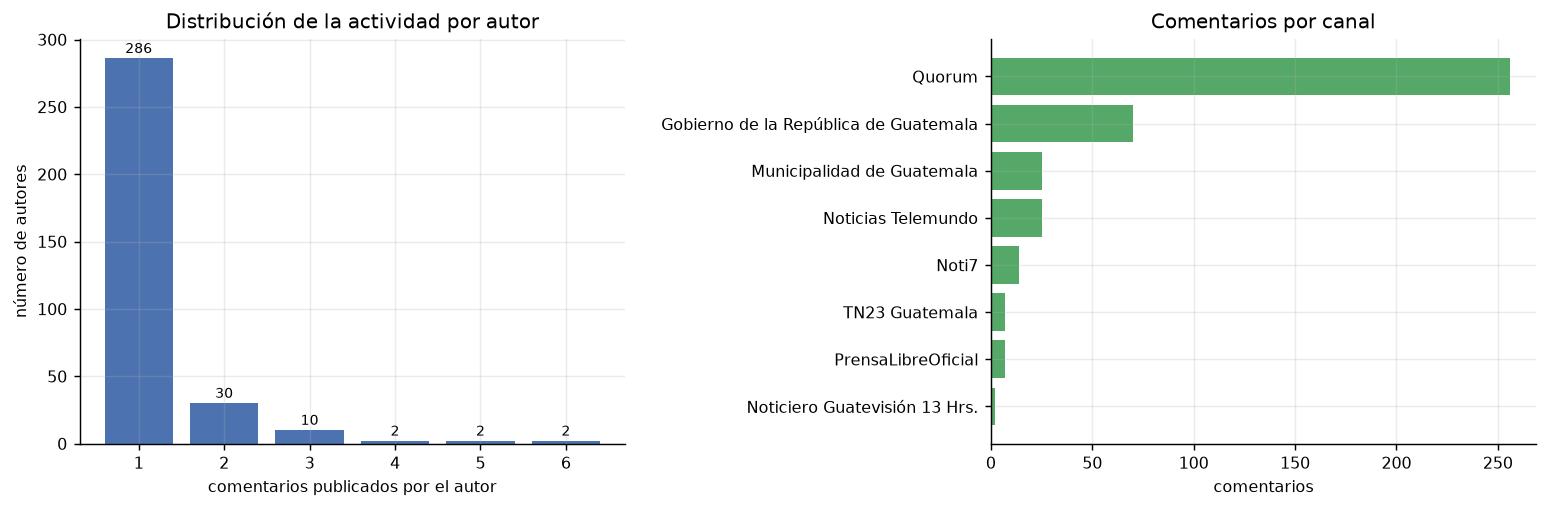
\includegraphics[width=\linewidth]{figuras/eda_autores_canales.png}
\caption{Distribuci\'on de la actividad por autor (izq.): decae de 286 autores con un comentario a
2 con seis. Comentarios por canal (der.): dominio de Quorum.}
\label{fig:autorescanales}
\end{figure}

\begin{figure}[H]
\centering
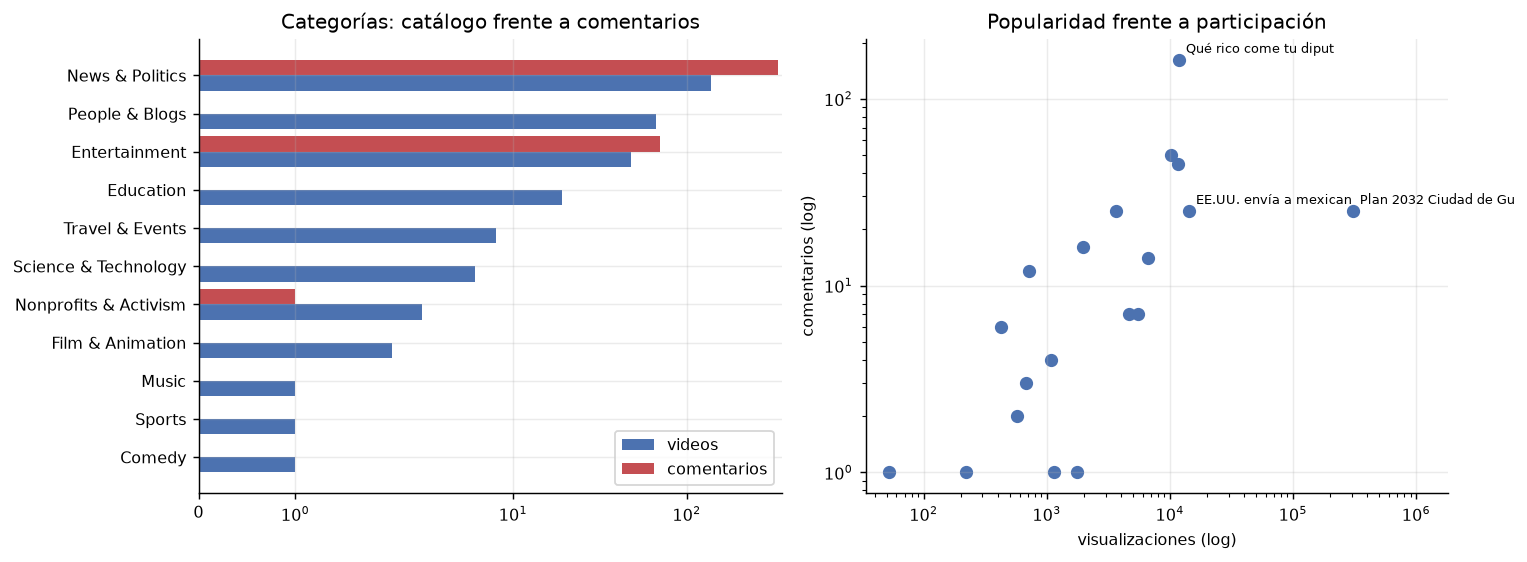
\includegraphics[width=\linewidth]{figuras/eda_categorias_pop.png}
\caption{Categor\'ias, cat\'alogo frente a comentarios (izq.): People \& Blogs, Education y
Travel \& Events tienen videos pero ninguna participaci\'on recolectada. Popularidad frente a
participaci\'on en escala log--log (der.): ``Plan 2032'' queda claramente por debajo de la tendencia.}
\label{fig:categorias}
\end{figure}

\begin{figure}[H]
\centering
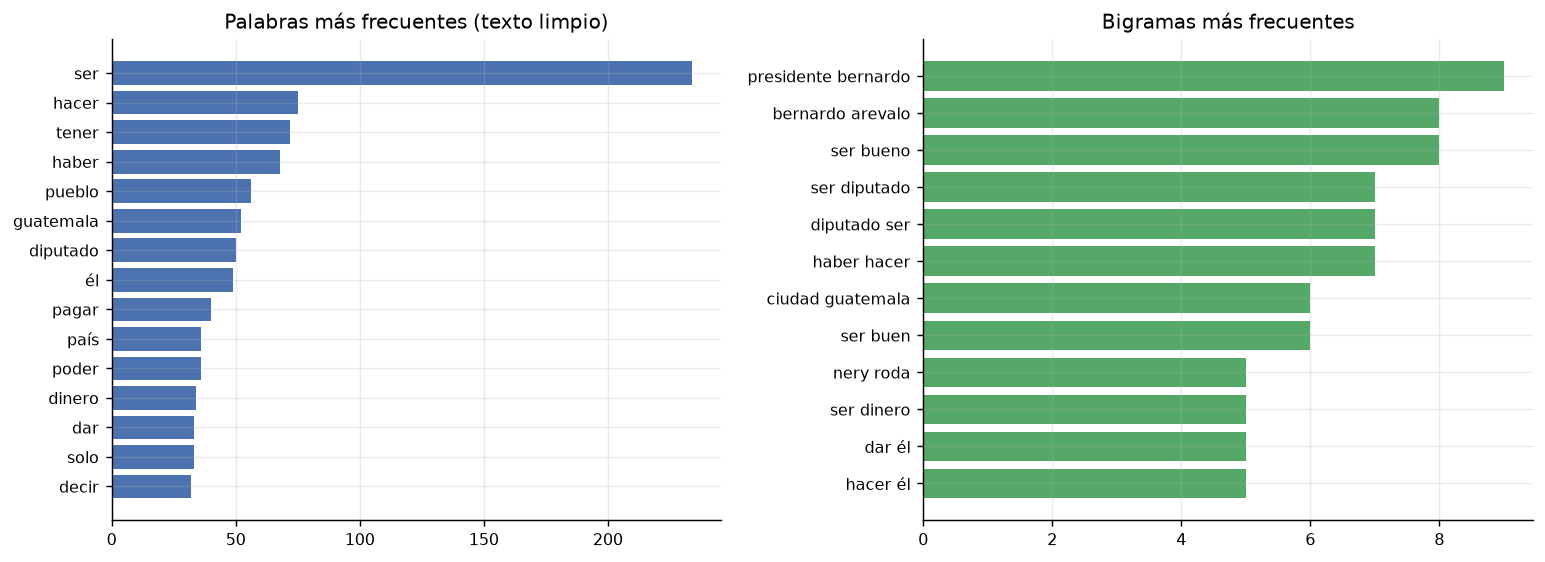
\includegraphics[width=\linewidth]{figuras/eda_palabras.png}
\caption{Palabras (izq.) y bigramas (der.) m\'as frecuentes en el texto limpio.}
\label{fig:palabras}
\end{figure}

\subsection{Preguntas obligatorias (inciso 3.5)}
\begin{description}[leftmargin=0em,style=unboxed,itemsep=3pt]
\item[\textnormal{\itshape \textquestiondown{}Qu\'e videos y canales concentran la mayor participaci\'on?}]
``Qu\'e rico come tu diputado'' con 161 comentarios (39.7\,\%) y, a nivel de canal, Quorum con 256
(63.1\,\%). Le siguen Gobierno de la Rep\'ublica (70) y un grupo de medios con 25 o menos.

\item[\textnormal{\itshape \textquestiondown{}Existen audiencias compartidas?}]
S\'i, pero muy poco. Solo 9 de 332 autores comentaron en m\'as de un video y el solapamiento entre
videos alcanza como m\'aximo 2 autores compartidos (entre ``Internet: escoger el menos malo'' y
``Arroz con pollo a la MONOPOLIO'', y entre ``La cooptaci\'on\dots'' y ``Qu\'e rico come tu
diputado''). Solo 11 de los 171 pares posibles de videos comparten al menos un autor.

\item[\textnormal{\itshape \textquestiondown{}Qu\'e autores funcionan como puentes?}]
Los nueve autores multivideo, y en particular los que cruzan canales distintos: \texttt{@virgiliogarcia3039}
(Gobierno$\leftrightarrow$Quorum), \texttt{@MarcosCarillo-b1r} (Quorum$\leftrightarrow$TN23),
\texttt{@franciscoflores3120} (Gobierno$\leftrightarrow$Noti7), \texttt{@moisesvaldez4043}
(PrensaLibre$\leftrightarrow$Quorum). Sin ellos, cada canal quedar\'ia como un grupo separado. Los dos
autores con m\'as videos son \texttt{@inge\_vergueta} y \texttt{@hashojea7348}, ambos con 3 videos y
solo dentro de Quorum.

\item[\textnormal{\itshape \textquestiondown{}Qu\'e temas y sentimientos caracterizan a los grupos?}]
Usando los videos como agrupamiento provisional y una polaridad por l\'exico, el corpus se divide en
dos bloques. El \textbf{bloque cr\'itico} (Quorum): vocabulario de \emph{diputado, pueblo, sueldo,
dinero, pacto corrupto} y la mayor proporci\'on de comentarios negativos (24\,\% en ``Qu\'e rico come
tu diputado'', 20\,\% en el video de la USAC). El \textbf{bloque institucional} (Municipalidad y
Gobierno): vocabulario de \emph{proyecto, ciudad, presidente, saludos} y polaridad mayoritariamente
positiva (64\,\% de positivos y ning\'un negativo en ``Plan 2032''). El an\'alisis formal est\'a en la
Secci\'on~\ref{sec:sentimiento}.

\item[\textnormal{\itshape \textquestiondown{}La visibilidad coincide con la participaci\'on?}]
Solo en parte. La correlaci\'on de rangos vistas--comentarios es alta (0.811), pero la tasa de
comentarios por mil vistas var\'ia en dos \'ordenes de magnitud y el video m\'as visto del subconjunto
es el que menos comenta en t\'erminos relativos. La visibilidad no explica qu\'e videos entraron a la
muestra.

\item[\textnormal{\itshape \textquestiondown{}Qu\'e conclusiones quedan limitadas por la recolecci\'on?}]
Pr\'acticamente todas las que involucren el cat\'alogo completo. El 93.5\,\% de los videos no tiene
comentarios recolectados, los 105 videos del grupo \texttt{official\_gov} tienen cero, y una sola
consulta aporta m\'as de la mitad de los comentarios. Cualquier afirmaci\'on sobre ``qu\'e temas
generan m\'as conversaci\'on en YouTube Guatemala'' estar\'ia midiendo la estrategia de \emph{scraping}.
\end{description}

\subsection{Preguntas adicionales (inciso 3.6)}
\begin{enumerate}[leftmargin=1.4em,itemsep=3pt]
\item \textbf{\textquestiondown{}Los videos con m\'as comentarios reciben m\'as ``me gusta''?} No necesariamente. La
correlaci\'on de rangos es alta (0.871), pero ``Plan 2032'' concentra el 73\,\% de todos los ``me
gusta'' con apenas el 6.2\,\% de los comentarios, mientras que el video m\'as comentado re\'une el
39.7\,\% de los comentarios y solo el 15.4\,\% de los ``me gusta''. Comentar exige redactar; reaccionar
no, y en este corpus se activan en videos distintos.
\item \textbf{\textquestiondown{}La cobertura de comentarios depende de la estrategia de recolecci\'on?} De forma
determinante. Los 105 videos de \texttt{official\_gov} no tienen ni un comentario recolectado pese a
una mediana de vistas comparable (521). \texttt{topic} aporta 363 comentarios y \texttt{channel} 43.
La ausencia de comentarios en m\'as del 90\,\% del cat\'alogo es un artefacto del dise\~no.
\item \textbf{\textquestiondown{}La extensi\'on del comentario var\'ia por canal?} S\'i. Quorum promedia 26.4 palabras
y Gobierno de la Rep\'ublica 25.7, mientras Noti7 promedia 9.6 y TN23 solo 7.0. Los videos de an\'alisis
pol\'itico generan intervenciones m\'as largas; las notas de nota roja generan reacciones breves. Debe
leerse con cuidado: los canales peque\~nos tienen muestras de 7 a 14 casos.
\end{enumerate}

\section{Construcci\'on de la red bipartita autor--video}

\subsection{Construcci\'on y definici\'on de aristas y pesos}
Se construy\'o un grafo \textbf{no dirigido} con dos conjuntos disjuntos de nodos: 332 autores
(\texttt{author\_channel\_id}) y 19 videos comentados (\texttt{video\_id}). Se crea una arista
autor--video cuando ese autor public\'o al menos un comentario en ese video, y el \textbf{peso} es el
n\'umero de comentarios que ese autor public\'o en ese video. Las 36 filas que son respuestas se
cuentan como participaci\'on normal del autor en el video: la arista describe presencia, no jerarqu\'ia
conversacional. Verificaci\'on: la suma de pesos es 406 = total de comentarios; el grafo es bipartito.

\subsection{Tabla de nodos y tabla de aristas}
Se entregan \texttt{nodos\_bipartita.csv} (351 filas $\times$ 15 columnas) y
\texttt{aristas\_bipartita.csv} (343 filas $\times$ 6 columnas).

\begin{table}[H]
\centering
\caption{Esquema de las tablas entregadas.}
\begin{tabular}{l p{11.2cm}}
\toprule
Tabla & Columnas \\
\midrule
Nodos & \texttt{id, etiqueta, tipo} (\texttt{autor}/\texttt{video}), \texttt{grado},
  \texttt{grado\_ponderado}, \texttt{comentarios, autores, videos, canales, likes, respuestas},
  \texttt{author\_handle} (autores), \texttt{channel\_name, view\_count, category} (videos). \\
Aristas & \texttt{origen} (autor), \texttt{destino} (video), \texttt{peso} (n\'um. de comentarios),
  \texttt{likes}, \texttt{respuestas}, \texttt{tipo\_arista} (\texttt{autor-video}). \\
\bottomrule
\end{tabular}
\end{table}

Distribuci\'on de pesos de las 343 aristas: 303 con peso 1, 28 con 2, 7 con 3, 1 con 4, 2 con 5 y
2 con 6. Nodos de mayor grado ponderado: los videos ``Qu\'e rico come tu diputado'' (128),
``La cooptaci\'on\dots'' (49) e ``Inician trabajos del Puente Belice II'' (32); del lado autor,
\texttt{@hashojea7348} e \texttt{@inge\_vergueta} con grado ponderado 4 y 3.

\subsection{Visualizaci\'on de la red completa}
\begin{figure}[H]
\centering
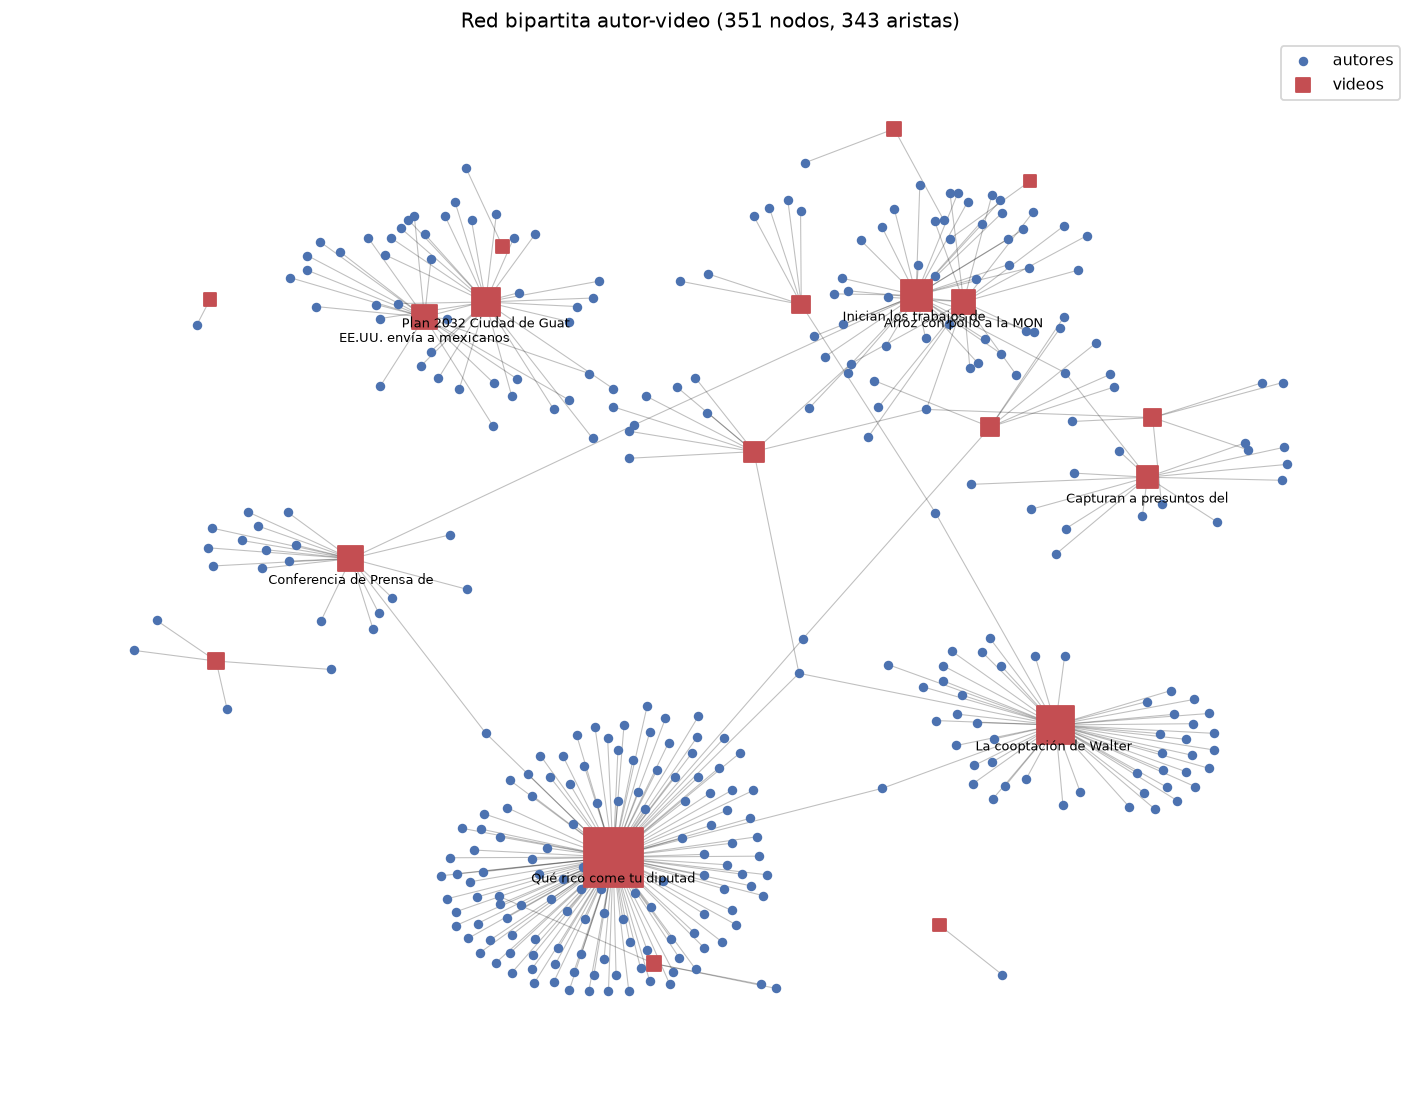
\includegraphics[width=0.96\linewidth]{figuras/red_bipartita.png}
\caption{Red bipartita autor--video: 351 nodos (332 autores en azul, 19 videos en rojo) y 343 aristas.
Cada video es el centro de una estrella de autores que solo aparecen ah\'i; las estrellas se unen
d\'ebilmente por los pocos autores puente.}
\label{fig:bipartita}
\end{figure}

\begin{figure}[H]
\centering
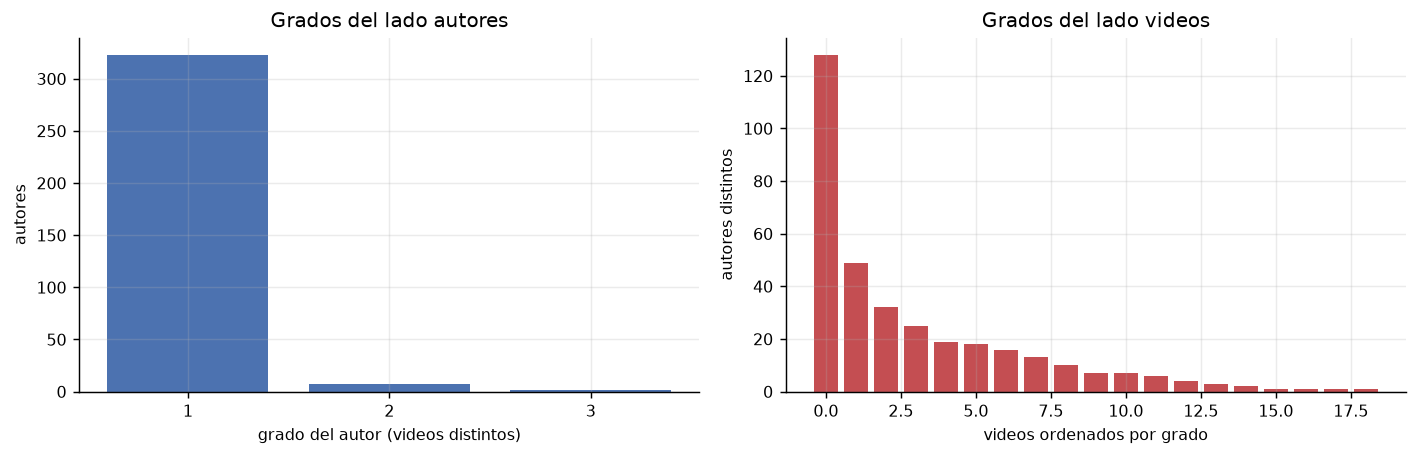
\includegraphics[width=\linewidth]{figuras/grados_bipartita.png}
\caption{Distribuci\'on de grados. Lado autores (izq.): 323 de 332 tienen grado 1. Lado videos (der.):
grado muy dispar, con un video que concentra 128 autores distintos.}
\label{fig:gradosbip}
\end{figure}

Densidad bipartita 0.054. Grado medio de autores \textbf{1.03} (m\'aximo 3), de videos \textbf{18.05}
(m\'aximo 128). La red se separa en \textbf{10 componentes conexas}: la mayor tiene \textbf{286 nodos
(81.5\,\%)} y agrupa 10 videos unidos exclusivamente por los autores multivideo; las otras nueve son
videos aislados con su propio p\'ublico. \textbf{Eliminar menos de diez autores puente fragmentar\'ia
la componente mayor por video.}

\subsection{Qu\'e significa una arista}
Una arista autor--video significa una sola cosa: ese autor public\'o al menos un comentario en ese
video, y el peso indica cu\'antos. \textbf{No} implica que el autor haya visto el video completo ni que
apruebe su contenido (buena parte de los comentarios son cr\'iticos). Dos autores conectados al mismo
video no son amigos, no se conocen y no necesariamente se leyeron: comparten un espacio de publicaci\'on,
no una conversaci\'on. La ausencia de arista tampoco es desinter\'es: 274 videos del cat\'alogo no
tienen aristas porque no se recolectaron sus comentarios. La red describe \emph{participaci\'on
observada}, no participaci\'on real.

\section{Proyecciones de la red}

\subsection{Construcci\'on de las proyecciones}
\textbf{Autor--autor:} dos autores se conectan si comentaron en el mismo video; el peso es el n\'umero
de videos compartidos. Resultado: 332 nodos y \textbf{10\,732} aristas (10\,730 con peso 1, solo 2 con
peso 2). \textbf{Video--video:} dos videos se conectan si comparten al menos un autor; el peso es el
n\'umero de autores compartidos. Resultado: 19 nodos y \textbf{11} aristas (9 con peso 1, 2 con peso 2).

\subsection{Comparaci\'on de las proyecciones}
\begin{table}[H]
\centering
\caption{Comparaci\'on de las dos proyecciones.}
\begin{tabular}{l r r}
\toprule
M\'etrica & Autor--autor & Video--video \\
\midrule
Nodos & 332 & 19 \\
Aristas & 10\,732 & 11 \\
Densidad & 0.195 & 0.064 \\
Grado medio & 64.65 & 1.16 \\
Componentes & 10 & 10 \\
Nodos aislados & 4 & 9 \\
\bottomrule
\end{tabular}
\end{table}

La proyecci\'on \textbf{autor--autor} representa \emph{coaudiencia}: casi todas sus aristas nacen de
autores que comentaron en el mismo video, de modo que cada video genera un \emph{clique} completo de
sus comentaristas. Por eso tiene decenas de miles de aristas y una transitividad casi perfecta, pero
esa densidad es un artefacto de la proyecci\'on, no evidencia de interacci\'on real. La proyecci\'on
\textbf{video--video} representa \emph{solapamiento de p\'ublico}: mide cu\'antos videos comparten
comentaristas. Es dispersa (solo 11 aristas) porque el solapamiento de audiencias entre videos es
m\'inimo. Cada proyecci\'on responde a una pregunta distinta: la primera, ``\textquestiondown{}qu\'e autores
coincidieron?''; la segunda, ``\textquestiondown{}qu\'e contenidos comparten audiencia?''.

\subsection{Visualizaci\'on de las proyecciones}
\begin{figure}[H]
\centering
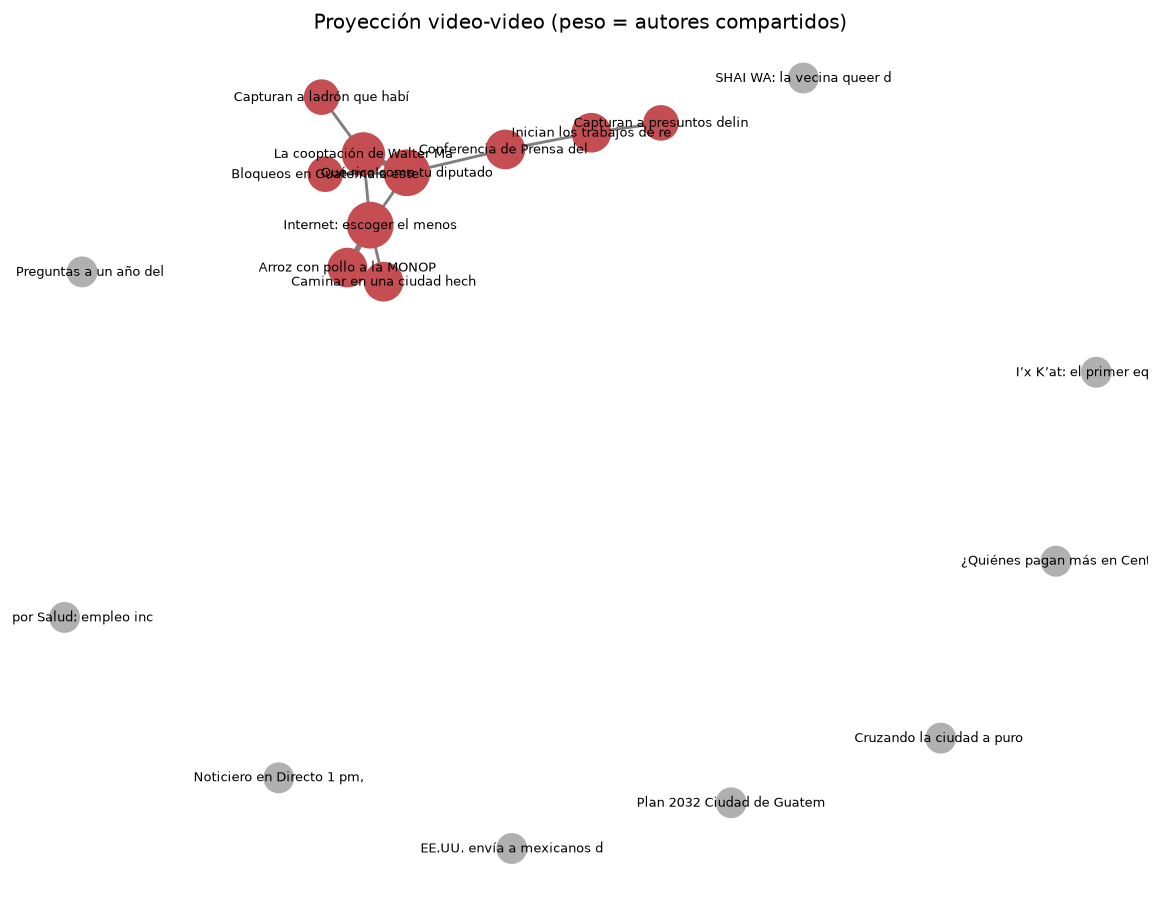
\includegraphics[width=0.82\linewidth]{figuras/proy_video.png}
\caption{Proyecci\'on video--video (grosor de arista = autores compartidos). Solo 10 de 19 videos
tienen alguna conexi\'on; 9 quedan aislados.}
\label{fig:proyvideo}
\end{figure}

\begin{figure}[H]
\centering
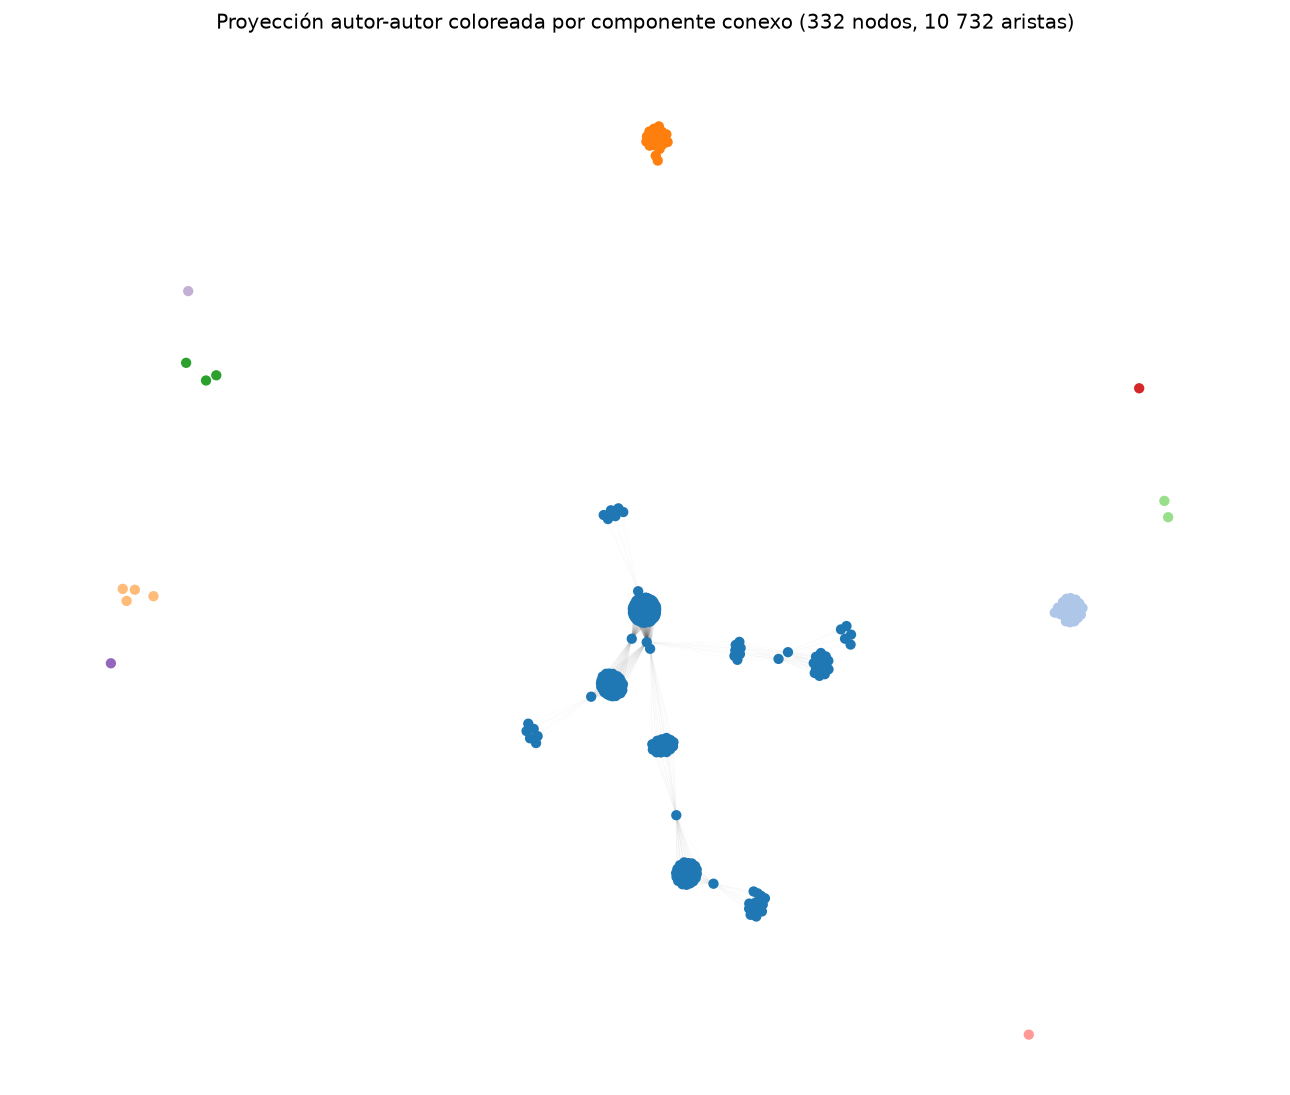
\includegraphics[width=0.86\linewidth]{figuras/proy_autor.png}
\caption{Proyecci\'on autor--autor coloreada por componente conexo (332 nodos, 10\,732 aristas). Cada
c\'umulo denso corresponde a los comentaristas de un mismo video.}
\label{fig:proyautor}
\end{figure}

\section{Topolog\'ia y fragmentaci\'on}

\subsection{Nodos, aristas, densidad, grado y componentes}
\begin{table}[H]
\centering
\caption{Resumen topol\'ogico de las tres redes.}
\begin{tabular}{l r r r r r r r r}
\toprule
Red & Nodos & Aristas & Dens. & $\bar{k}$ & $k_{\max}$ & Comp. & Comp.\ mayor & \% mayor \\
\midrule
Bipartita autor--video & 351 & 343 & 0.054 & 1.95 & 128 & 10 & 286 & 81.5 \\
Proyecci\'on autor--autor & 332 & 10\,732 & 0.195 & 64.65 & 183 & 10 & 276 & 83.1 \\
Proyecci\'on video--video & 19 & 11 & 0.064 & 1.16 & 4 & 10 & 10 & 52.6 \\
\bottomrule
\end{tabular}
\end{table}

\begin{figure}[H]
\centering
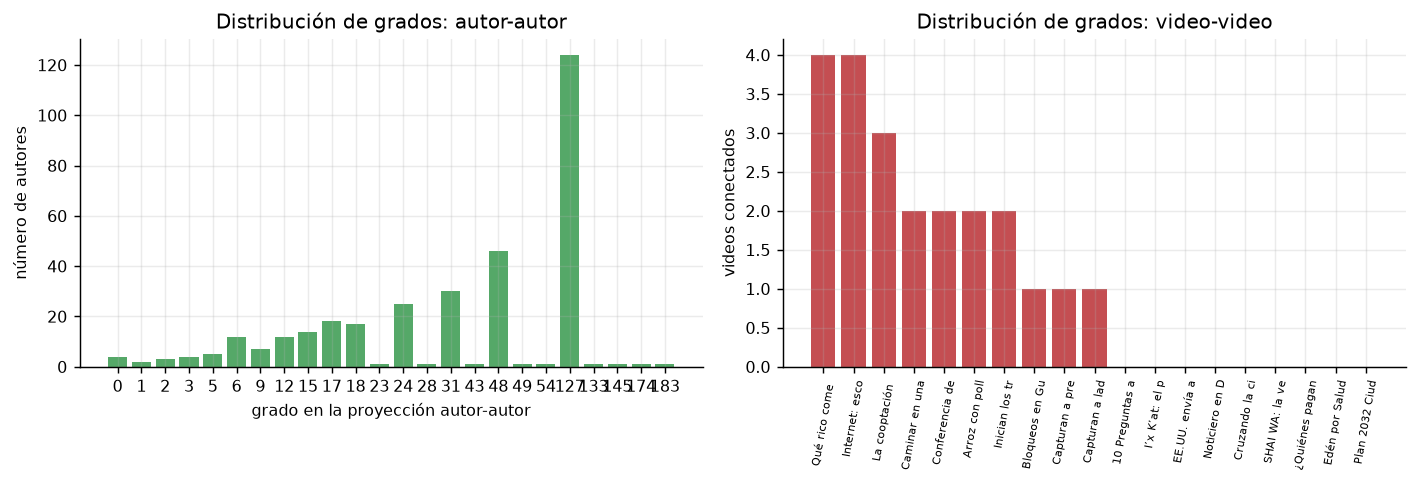
\includegraphics[width=\linewidth]{figuras/grados_proy.png}
\caption{Distribuci\'on de grados en las proyecciones. Autor--autor (izq.): grados altos por el efecto
\emph{clique}. Video--video (der.): grados $\leq 4$, muchos videos con grado 0.}
\label{fig:gradosproy}
\end{figure}

La distribuci\'on de grados est\'a fuertemente sesgada en la bipartita: la mayor\'ia de los nodos
(los autores) tiene pocas conexiones y el grado est\'a concentrado en unos pocos videos.

\subsection{Cohesi\'on y transitividad}
\begin{table}[H]
\centering
\caption{Cohesi\'on y transitividad.}
\begin{tabular}{l r r r r}
\toprule
Red & Transit.\ global & Clustering medio & Di\'ametro (comp.\ mayor) & Dist.\ media \\
\midrule
Bipartita autor--video & 0.000 & 0.000 & 12 & 4.715 \\
Proyecci\'on autor--autor & 0.984 & 0.972 & 6 & 2.356 \\
Proyecci\'on video--video & 0.316 & 0.149 & 5 & 2.489 \\
\bottomrule
\end{tabular}
\end{table}
La transitividad de la bipartita es \textbf{0 por construcci\'on} (no hay tri\'angulos en un grafo
bipartito). En la proyecci\'on autor--autor es casi 1 por el efecto \emph{clique}, no por cohesi\'on
social genuina. En la proyecci\'on video--video, 0.316 indica que cuando dos videos comparten p\'ublico
con un tercero, a veces (pero no siempre) tambi\'en lo comparten entre s\'i.

\subsection{Nodos, videos y grupos perif\'ericos o aislados}
\textbf{Aislamiento observado (dentro de la red):} 323 de 332 autores (97.3\,\%) tienen grado 1 en la
bipartita; 4 autores quedan aislados en la proyecci\'on autor--autor (comentaron en videos sin ning\'un
coautor); 9 de 19 videos quedan aislados en la proyecci\'on video--video.
\textbf{Ausencia de datos (fuera de la red):} 274 de 293 videos del cat\'alogo (93.5\,\%) no aparecen
como nodos porque no se recolectaron sus comentarios, \textbf{no} porque se haya observado que carecen
de audiencia. La distinci\'on es esencial: el primer grupo es un resultado, el segundo es una
limitaci\'on de cobertura.

\subsection{Interpretaci\'on de los hallazgos estructurales}
La topolog\'ia confirma y precisa lo visto en el an\'alisis exploratorio:
\begin{itemize}[leftmargin=1.4em,itemsep=2pt]
\item \textbf{Estructura de estrellas.} El grado medio de autores (1.03) frente al de videos (18.05)
y la transitividad nula de la bipartita describen un grafo donde cada video es un centro y los autores
son hojas. No hay comunidades de discusi\'on: hay audiencias yuxtapuestas.
\item \textbf{Fragmentaci\'on alta y cohesi\'on fr\'agil.} Diez componentes; la mayor cubre el 81.5\,\%
pero su conectividad depende de $<10$ autores puente. El di\'ametro 12 y la distancia media 4.7 en la
bipartita indican que incluso dentro de la componente mayor los videos est\'an ``lejos'' entre s\'i:
para ir de un video a otro hay que pasar por un autor puente y otro video.
\item \textbf{Las proyecciones enga\~nan si se leen sin contexto.} La autor--autor parece una red
social densa (densidad 0.195, clustering 0.97) pero esa densidad es mec\'anica. La video--video, que
s\'i mide un fen\'omeno real (solapamiento de p\'ublico), es casi vac\'ia: las audiencias de estos
videos apenas se tocan.
\item \textbf{El aislamiento observado es real; la ausencia de datos, no.} Se puede afirmar que estos
332 autores rara vez comentan en m\'as de un video; no se puede afirmar nada sobre los 274 videos sin
datos.
\end{itemize}

\section{Comunidades}

\subsection{Selecci\'on de la red y justificaci\'on}
Se detectan comunidades sobre la \textbf{red bipartita autor--video ponderada}, no sobre las
proyecciones. Razones: (i) la proyecci\'on autor--autor est\'a formada por \emph{cliques} de video, de
modo que cualquier algoritmo recuperar\'ia trivialmente ``un grupo por video'' y la modularidad
resultante ser\'ia un artefacto; (ii) la proyecci\'on video--video tiene solo 11 aristas y 9 nodos
aislados, insuficiente para una partici\'on informativa; (iii) la bipartita conserva toda la
informaci\'on (qui\'en comenta d\'onde y cu\'antas veces) y permite que los autores puente unan
comunidades en lugar de forzar una por video. Louvain admite grafos bipartitos ponderados aunque no
fue dise\~nado espec\'ificamente para ellos; se acepta esta limitaci\'on y se interpreta el resultado
en consecuencia.

\subsection{Algoritmo aplicado}
Se aplic\'o \textbf{Louvain} (\texttt{networkx.algorithms.community.louvain\_communities}) con
\texttt{weight='weight'}, \texttt{resolution=1.0} y \texttt{seed=7} para reproducibilidad. Louvain
optimiza la \textbf{modularidad} de forma voraz y jer\'arquica. Supuestos: las comunidades son
disjuntas (cada nodo pertenece a una sola) y densamente conectadas hacia dentro respecto a un modelo
nulo de configuraci\'on. \textbf{Tratamiento de los pesos:} el peso (n\'umero de comentarios de un
autor en un video) entra directamente en la modularidad, de modo que un autor que comenta muchas
veces en un video queda m\'as firmemente ligado a su comunidad.

\subsection{N\'umero de comunidades, tama\~nos y calidad}
\begin{table}[H]
\centering
\caption{Comunidades detectadas con Louvain.}
\begin{tabular}{l r}
\toprule
N\'umero de comunidades & 17 \\
Modularidad & 0.777 \\
Tama\~nos & 126, 48, 32, 31, 26, 19, 19, 14, 8, 8, 5, 4, 3, 2, 2, 2, 2 \\
\bottomrule
\end{tabular}
\end{table}
La modularidad 0.777 es alta, lo que confirma que la red se separa muy bien en bloques. Esto era
esperable dada la estructura de estrellas: casi cada comunidad coincide con el p\'ublico de un video.

\begin{figure}[H]
\centering
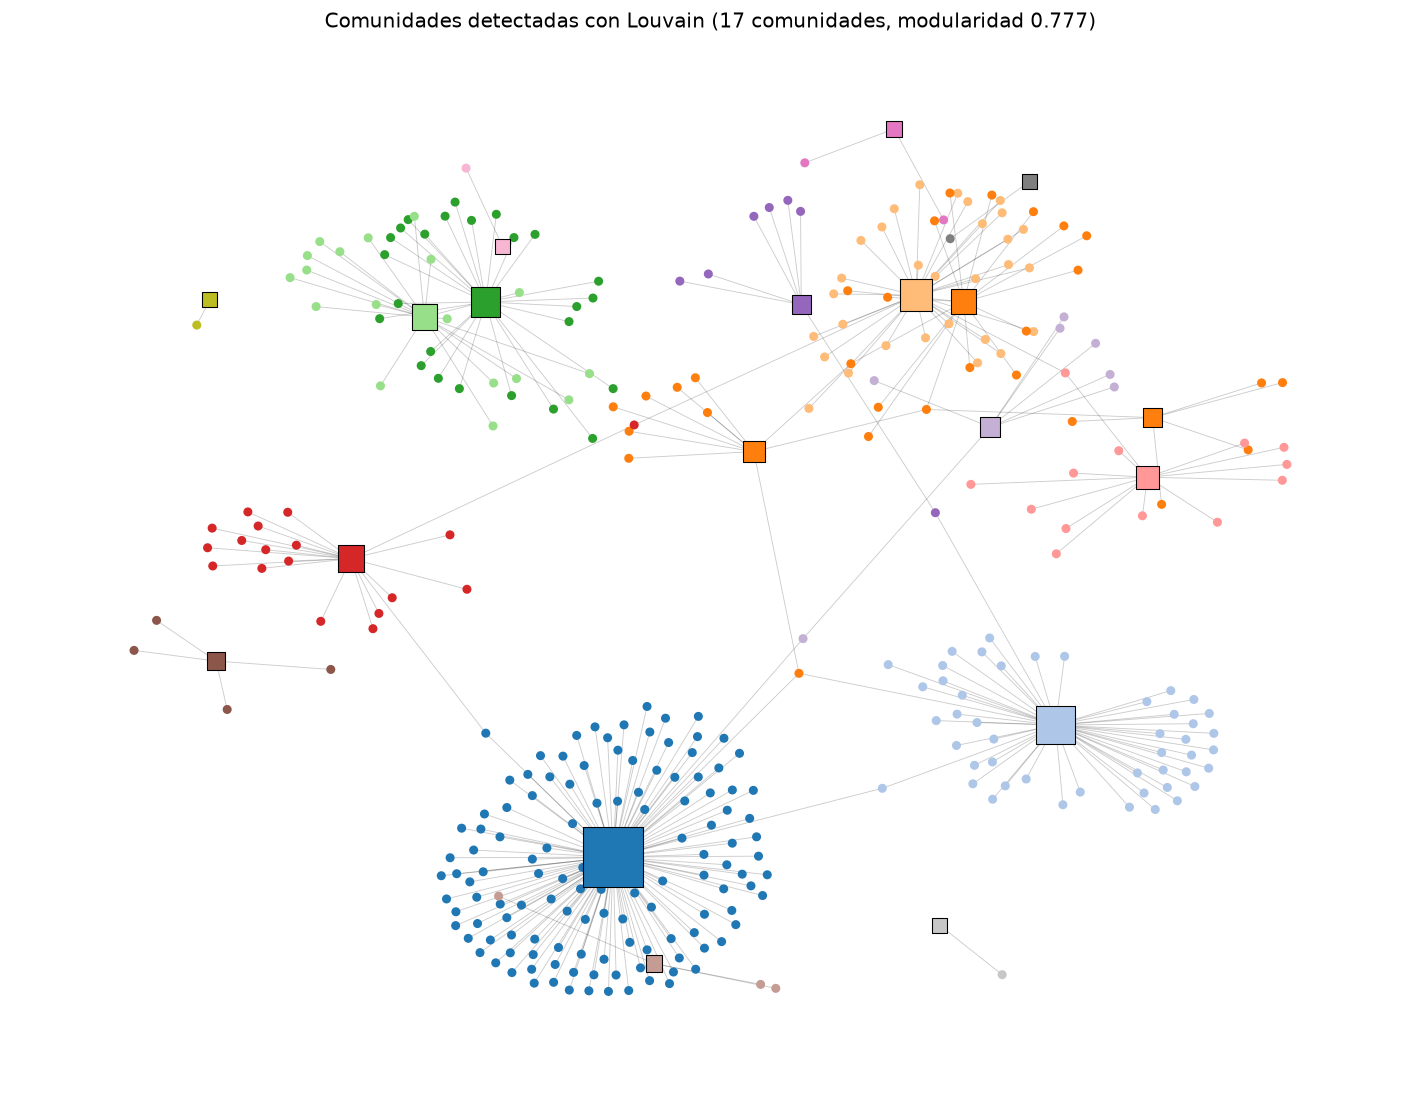
\includegraphics[width=0.96\linewidth]{figuras/comunidades.png}
\caption{Comunidades detectadas con Louvain (17 comunidades, modularidad 0.777). Los cuadrados son
videos, los c\'irculos autores; el color indica la comunidad.}
\label{fig:comunidades}
\end{figure}

\subsection{Caracterizaci\'on de las tres comunidades principales}
\begin{table}[H]
\centering
\caption{Las tres comunidades m\'as grandes.}
\small
\begin{tabular}{l p{2.2cm} r r p{3.2cm} p{3.0cm}}
\toprule
Com. & Videos (canal) & Aut. & Coment. & Temas frecuentes & Sentimiento \\
\midrule
1 & ``Qu\'e rico come tu diputado'' (Quorum) & 125 & 161 &
  pueblo, diputado, pagar & 65\,\% neutral, 24\,\% negativo, 11\,\% positivo \\
2 & ``La cooptaci\'on de W. Mazariegos en la USAC'' (Quorum) & 47 & 50 &
  corrupto, universidad & 64\,\% neutral, 20\,\% negativo, 16\,\% positivo \\
3 & 3 videos de Quorum (movilidad, internet, mercado) & 29 & $\sim$34 &
  excelente, ciudad, internet & 47\,\% neutral, 47\,\% positivo, 6\,\% negativo \\
\bottomrule
\end{tabular}
\end{table}

La \textbf{Comunidad 1} es, por s\'i sola, casi tan grande como el resto: re\'une 161 comentarios,
sentimiento mayoritariamente neutral con un 24\,\% de negativos (por encima del 15.5\,\% general).
La \textbf{Comunidad 2} gira en torno a ``corrupto'' y la universidad, con perfil de sentimiento
similar. La \textbf{Comunidad 3} es la \'unica que fusiona m\'as de un video, producto de los autores
puente; su sentimiento es mucho m\'as equilibrado y aparece ``excelente'' entre las palabras
frecuentes, lo que sugiere una audiencia distinta, m\'as af\'in al canal, que comenta varios videos
con tono elogioso en lugar de cr\'itico.

\section{Nodos centrales y participantes puente}

\subsection{Medidas de centralidad y su justificaci\'on}
Se calcularon tres medidas complementarias sobre la red bipartita:
\begin{itemize}[leftmargin=1.4em,itemsep=2pt]
\item \textbf{Intermediaci\'on (betweenness)}, no ponderada y normalizada: mide cu\'antos caminos
m\'as cortos pasan por un nodo. Es la medida clave para identificar \emph{puentes}: en una red
fragmentada como esta, los nodos con betweenness alto son los que mantienen conectada la componente
mayor.
\item \textbf{PageRank} ponderado por el peso de las aristas: mide importancia recursiva y absorbe
bien la asimetr\'ia de grado; identifica los videos y autores que reciben ``m\'as flujo'' de
participaci\'on.
\item \textbf{Centralidad de vector propio}, calculada solo sobre la componente mayor (no est\'a
definida en un grafo desconectado): mide estar conectado a nodos que a su vez est\'an bien conectados.
\end{itemize}
No se report\'o cercan\'ia global porque la red est\'a desconectada; el di\'ametro y la distancia media
ya se reportaron en la Secci\'on~6.2.

\subsection{Interpretaci\'on separada para autores y videos}
\textbf{Videos --- alcance y capacidad de conectar audiencias.} PageRank e intermediaci\'on coinciden
en el mismo orden: ``Qu\'e rico come tu diputado'' (PageRank 0.167, betweenness 0.566), ``La
cooptaci\'on\dots'' (0.063 / 0.227), ``Inician trabajos del Puente Belice II'' (0.043 / 0.188) y
``Conferencia de Prensa del Gobierno'' (0.025 / 0.244). Los dos primeros dominan por volumen de
comentaristas; los dos siguientes tienen betweenness alto relativo a su tama\~no porque est\'an
pegados a autores puente que conectan Quorum con Gobierno.

\textbf{Autores --- recurrencia y diversidad.} Solo \textbf{9 de 332 autores} tienen betweenness $>0$;
son exactamente los autores multivideo. Los de mayor intermediaci\'on son \texttt{@virgiliogarcia3039}
(3 coment., 2 videos, betweenness 0.232), \texttt{@inge\_vergueta} (3 coment., 3 videos, 0.218) y
\texttt{@josegil3813} (2 coment., 2 videos, 0.177). La recurrencia (comentar mucho) y la diversidad
(comentar en varios videos) no coinciden: \texttt{@hashojea7348} tiene 4 comentarios pero betweenness
bajo (0.060) porque sus 3 videos son todos de Quorum y no conectan bloques distintos.

\subsection{Participantes recurrentes, autores puente y videos articuladores}
En la componente mayor (286 nodos) hay \textbf{17 puntos de articulaci\'on}: \textbf{7 autores} y
\textbf{los 10 videos}. Que los 10 videos sean puntos de articulaci\'on es la firma de la estructura
de estrellas: quitar cualquier video desconecta a todos sus comentaristas exclusivos. Los 7 autores
articuladores (\texttt{@franciscoflores3120}, \texttt{@josegil3813}, \texttt{@virgiliogarcia3039},
\texttt{@moisesvaldez4043}, \texttt{@hashojea7348}, \texttt{@inge\_vergueta},
\texttt{@MarcosCarillo-b1r}) son los que, si se eliminan, parten la componente mayor en trozos por
video. \textbf{La conectividad global de la red depende de siete personas.}

\section{An\'alisis de contenido y sentimiento}
\label{sec:sentimiento}

\subsection{M\'etodo de an\'alisis de sentimiento y su justificaci\'on}
Se clasific\'o cada comentario en \texttt{positivo}, \texttt{negativo} o \texttt{neutral} con un
\textbf{l\'exico de polaridad en espa\~nol adaptado al dominio}. El procedimiento normaliza el texto
original (min\'usculas y eliminaci\'on de tildes), cuenta ocurrencias de dos listas de palabras
(una positiva: \emph{excelente, gracias, felicidades, apoyo, esperanza, orgullo\dots}; una negativa:
\emph{corrupto, ladr\'on, mentira, p\'esimo, fraude, impunidad, verg\"uenza\dots}) y asigna la
polaridad por mayor\'ia; el empate se resuelve como \texttt{neutral}.

\textbf{Justificaci\'on de la elecci\'on:}
\begin{itemize}[leftmargin=1.4em,itemsep=2pt]
\item \textbf{Tama\~no del corpus.} Con 406 comentarios no hay datos para entrenar ni validar un
clasificador supervisado; un m\'etodo basado en l\'exico no requiere entrenamiento.
\item \textbf{Dominio.} El corpus es de comentarios pol\'iticos guatemaltecos. Los l\'exicos y modelos
gen\'ericos (entrenados sobre rese\~nas de productos o tuits gen\'ericos) subestiman se\~nales
locales como ``pacto corrupto'', ``impunidad'' o ``inepto''. Una lista curada a mano permite incorporar
ese vocabulario.
\item \textbf{Reproducibilidad e interpretabilidad.} El l\'exico corre sin GPU, es determinista y cada
clasificaci\'on es auditable (se sabe exactamente qu\'e palabra la produjo), lo que es deseable en un
laboratorio.
\item \textbf{Consistencia con la limpieza.} Se aplica sobre \texttt{texto\_original}, conservando
may\'usculas, signos y emojis que la versi\'on lematizada elimina.
\end{itemize}

\textbf{Limitaciones reconocidas del m\'etodo:} no maneja negaci\'on (``no es corrupto'' se cuenta como
negativo), ni intensidad, ni iron\'ia; sobre-asigna la clase \texttt{neutral} cuando el comentario no
contiene palabras del l\'exico (61.6\,\% de los casos); y las listas, al ser manuales, tienen cobertura
incompleta. Un modelo transformer en espa\~nol (por ejemplo BETO afinado, o \texttt{pysentimiento})
dar\'ia una clasificaci\'on m\'as fina y es la extensi\'on natural de este trabajo; los resultados que
siguen deben leerse como una aproximaci\'on de primer orden.

\subsection{Distribuci\'on general y comparaci\'on por video, canal y comunidad}
\begin{table}[H]
\centering
\caption{Distribuci\'on general de sentimiento (406 comentarios).}
\begin{tabular}{l r r}
\toprule
Polaridad & Comentarios & Proporci\'on \\
\midrule
Neutral & 250 & 61.6\,\% \\
Positivo & 93 & 22.9\,\% \\
Negativo & 63 & 15.5\,\% \\
\bottomrule
\end{tabular}
\end{table}

\begin{table}[H]
\centering
\caption{Sentimiento por video (videos con $\geq 10$ comentarios).}
\small
\begin{tabular}{l r r r r}
\toprule
Video & $n$ & Neg. & Neutral & Pos. \\
\midrule
Qu\'e rico come tu diputado & 161 & 0.24 & 0.65 & 0.11 \\
La cooptaci\'on de W. Mazariegos en la USAC & 50 & 0.20 & 0.64 & 0.16 \\
Inician trabajos del Puente Belice II & 45 & 0.16 & 0.49 & 0.36 \\
Conferencia de Prensa del Gobierno & 25 & 0.04 & 0.68 & 0.28 \\
EE.UU.\ env\'ia a mexicanos deportados & 25 & 0.08 & 0.72 & 0.20 \\
Plan 2032 Ciudad de Guatemala & 25 & 0.00 & 0.36 & 0.64 \\
Arroz con pollo a la MONOPOLIO & 16 & 0.06 & 0.56 & 0.38 \\
Capturan a presuntos delincuentes\dots & 14 & 0.00 & 0.86 & 0.14 \\
Internet: escoger el menos malo & 12 & 0.08 & 0.42 & 0.50 \\
\bottomrule
\end{tabular}
\end{table}

\begin{table}[H]
\centering
\caption{Sentimiento por canal (canales con $\geq 10$ comentarios).}
\small
\begin{tabular}{l r r r r}
\toprule
Canal & $n$ & Neg. & Neutral & Pos. \\
\midrule
Quorum & 256 & 0.20 & 0.62 & 0.17 \\
Gobierno de la Rep\'ublica de Guatemala & 70 & 0.11 & 0.56 & 0.33 \\
Municipalidad de Guatemala & 25 & 0.00 & 0.36 & 0.64 \\
Noticias Telemundo & 25 & 0.08 & 0.72 & 0.20 \\
Noti7 & 14 & 0.00 & 0.86 & 0.14 \\
\bottomrule
\end{tabular}
\end{table}

\subsection{Hallazgos de contenido y sentimiento}
\begin{itemize}[leftmargin=1.4em,itemsep=2pt]
\item \textbf{El corpus es predominantemente neutral} (61.6\,\%), en parte real (muchos comentarios
son preguntas, datos o etiquetados de terceros) y en parte un efecto del m\'etodo, que marca neutral
todo comentario sin palabras del l\'exico.
\item \textbf{La polaridad depende del emisor, no del tema en abstracto.} Los videos de Quorum
concentran la negatividad (20\,\% negativo, 24\,\% en el video de los diputados); los de la
Municipalidad de Guatemala no tienen ni un comentario negativo y son 64\,\% positivos. Un mismo asunto
--- pol\'itica y gesti\'on p\'ublica --- produce comentarios cr\'iticos cuando lo publica un medio de
fiscalizaci\'on y comentarios de felicitaci\'on cuando lo publica la instituci\'on aludida.
\item \textbf{El vocabulario acompa\~na al sentimiento.} En las comunidades cr\'iticas dominan
\emph{diputado, pueblo, pagar, dinero, corrupto}; en las institucionales, \emph{proyecto, ciudad,
excelente, felicidades}. Los bigramas m\'as frecuentes del corpus (\emph{pacto corrupto},
\emph{bernardo arevalo}, \emph{diputado ser}) confirman que el eje tem\'atico es la pol\'itica
nacional.
\item \textbf{Los ``me gusta'' refuerzan el contenido positivo institucional:} ``Plan 2032'' concentra
el 73\,\% de los ``me gusta'' del corpus con un 64\,\% de comentarios positivos, mientras el video m\'as
comentado (cr\'itico) recibe muchos comentarios pero pocas reacciones.
\item \textbf{Cautela por tama\~no de muestra:} la comparaci\'on por canal solo es s\'olida para
Quorum ($n=256$) y Gobierno ($n=70$); los dem\'as canales tienen 14--25 comentarios y sus porcentajes
son orientativos.
\end{itemize}

\section{Interpretaci\'on, limitaciones y conclusiones}

\subsection{Los hallazgos en el contexto de participaci\'on y consumo en YouTube}
El retrato que emerge es coherente con lo que se sabe del consumo de contenido en plataformas de video:
una minor\'ia muy activa produce la mayor parte del texto y una mayor\'ia silenciosa (o de una sola
intervenci\'on) constituye el grueso de la audiencia. En estos datos, el 86\,\% de los autores comenta
una \'unica vez y tres videos concentran el 63\,\% de los comentarios. La participaci\'on por escrito
se organiza alrededor de \textbf{piezas de contenido}, no de \textbf{comunidades de usuarios}: la gente
llega a un video, comenta y no vuelve a cruzarse con los dem\'as comentaristas en otro video. Esto
explica por qu\'e la red bipartita tiene forma de estrellas y por qu\'e su cohesi\'on depende de un
pu\~nado de usuarios recurrentes.

Tambi\'en se observa que \textbf{comentar y reaccionar son conductas distintas}: los videos que
concentran comentarios (an\'alisis pol\'itico cr\'itico) no son los que concentran ``me gusta''
(comunicaci\'on institucional positiva). Y el tono del comentario est\'a fuertemente condicionado por
qui\'en publica el video: los medios de fiscalizaci\'on atraen cr\'itica, las instituciones atraen
felicitaciones. La conversaci\'on observada es, en su mayor parte, pol\'itica nacional guatemalteca
(diputados, presidente Ar\'evalo, pacto de corruptos, USAC).

\subsection{Limitaciones}
\begin{enumerate}[leftmargin=1.6em,itemsep=3pt]
\item \textbf{Cobertura de comentarios.} Solo 19 de 293 videos (6.5\,\%) tienen comentarios
recolectados y el n\'umero de comentarios por video parece topado por el \emph{scraping}
(m\'aximo 161). No se conoce el volumen real de conversaci\'on de ning\'un video, ni si los
comentarios recolectados son los primeros, los m\'as votados o una muestra sesgada.
\item \textbf{Selecci\'on por consultas.} Una sola consulta (\texttt{@quorumgt/videos}) aporta 231 de
406 comentarios, y el grupo \texttt{official\_gov} (105 videos) no aporta ninguno. El corpus refleja
la estrategia de b\'usqueda del recolector, no la actividad de la plataforma.
\item \textbf{Fechas relativas.} \texttt{published\_time} y \texttt{published\_text} (``hace 2 d\'ias'',
``hace 3 meses'') dependen del momento de recolecci\'on y no permiten ordenar eventos con precisi\'on
ni construir series temporales. La \'unica fecha absoluta, \texttt{publish\_date}, existe solo para
videos.
\item \textbf{Conteos observados al momento de recolecci\'on.} \texttt{view\_count} y
\texttt{like\_count} son fotograf\'ias de un instante; \texttt{view\_count} es acumulado desde la
publicaci\'on mientras que el conteo de comentarios es un tope de muestreo. Compararlos mezcla dos
escalas temporales distintas.
\item \textbf{Falta de relaciones expl\'icitas entre autores.} Los datos no permiten saber qui\'en
respondi\'o a qui\'en: \texttt{reply\_count} no identifica autores y solo 36 de las 51 respuestas
declaradas est\'an presentes. Toda la estructura de red se basa en \emph{coparticipaci\'on}
(comentar en el mismo video), no en interacci\'on directa.
\item \textbf{Concentraci\'on de comentarios en pocos videos.} El Gini sobre el cat\'alogo completo es
0.978. Cualquier estad\'istico agregado est\'a dominado por dos o tres videos de un solo canal (Quorum),
de modo que ``el comportamiento promedio'' del corpus es en realidad el comportamiento de esos videos.
\end{enumerate}

\subsection{Descripci\'on, asociaci\'on e inferencia}
\begin{itemize}[leftmargin=1.4em,itemsep=2pt]
\item \textbf{Descripci\'on} (lo que los datos dicen directamente): hay 406 comentarios de 332 autores
en 19 videos de 8 canales; el 39.7\,\% de los comentarios est\'a en un video; el 15.5\,\% de los
comentarios se clasific\'o como negativo; hay 7 autores cuya eliminaci\'on fragmenta la componente
mayor.
\item \textbf{Asociaci\'on} (relaciones observadas en \emph{esta} muestra, sin causalidad): a mayor
n\'umero de vistas, mayor n\'umero de comentarios entre los 19 videos ($\rho=0.811$); los videos de
Quorum se asocian con m\'as comentarios negativos que los de la Municipalidad; los comentarios m\'as
largos se asocian con canales de an\'alisis pol\'itico.
\item \textbf{Inferencia} (lo que \emph{no} se puede concluir): no se puede afirmar que el video
cr\'itico ``genere'' negatividad, ni que los usuarios de YouTube en Guatemala se comporten as\'i, ni
que la poblaci\'on guatemalteca opine lo que opinan estos 332 autores. La muestra no es aleatoria ni
representativa: es el resultado de un conjunto concreto de consultas sobre un conjunto concreto de
canales. Los resultados describen este corpus y no se generalizan.
\end{itemize}

\subsection{Conclusiones integradas}
\begin{enumerate}[leftmargin=1.6em,itemsep=3pt]
\item \textbf{Estructura.} La participaci\'on escrita observada se organiza como estrellas
video--comentaristas d\'ebilmente unidas. La red bipartita tiene 351 nodos y 343 aristas, densidad
0.054, grado medio de autores 1.03 y transitividad 0. Se fragmenta en 10 componentes; la mayor
(81.5\,\% de los nodos) se sostiene sobre menos de diez autores puente, de los cuales 7 son puntos de
articulaci\'on.
\item \textbf{Comunidades.} Louvain encuentra 17 comunidades con modularidad 0.777, pero esa nitidez
es consecuencia de la estructura de estrellas: cada comunidad es, esencialmente, el p\'ublico de un
video. La \'unica comunidad que fusiona varios videos lo hace gracias a los autores puente y tiene un
tono marcadamente m\'as positivo que las dem\'as.
\item \textbf{Centralidad.} Los nodos clave son pocos y claros: dos videos de Quorum concentran alcance
y PageRank; siete autores recurrentes concentran toda la intermediaci\'on. La influencia en esta red
no es difusa, es puntual.
\item \textbf{Contenido y sentimiento.} El corpus es pol\'itica nacional y es mayoritariamente neutral
(61.6\,\%), con un 15.5\,\% negativo y un 22.9\,\% positivo. La polaridad la determina el emisor del
video: los medios de fiscalizaci\'on atraen cr\'itica (Quorum, 20\,\% negativo) y las instituciones
atraen felicitaciones (Municipalidad, 64\,\% positivo, 0\,\% negativo).
\item \textbf{Limitaciones.} Todo lo anterior describe un subconjunto sesgado por el procedimiento de
recolecci\'on: el 93.5\,\% del cat\'alogo no aporta comentarios y una consulta aporta m\'as de la
mitad. Las conclusiones son v\'alidas para este corpus y no se extienden a YouTube ni a Guatemala.
La estructura de red se basa en coparticipaci\'on, no en interacci\'on directa, y el an\'alisis de
sentimiento es una aproximaci\'on por l\'exico que conviene refinar con un modelo transformer en
espa\~nol en trabajo futuro.
\end{enumerate}

\section*{Reproducibilidad}
El an\'alisis completo est\'a en el notebook \texttt{Laboratorio6\_DS\_Grupo7.ipynb}. Dependencias en
\texttt{requirements.txt} (\texttt{pandas}, \texttt{numpy}, \texttt{scipy}, \texttt{matplotlib},
\texttt{networkx}, \texttt{nltk}, \texttt{spacy} con \texttt{es\_core\_news\_sm}, \texttt{emoji}).
Ejecuci\'on: \texttt{uv venv \&\& uv pip install -r requirements.txt} y correr el notebook de arriba
abajo. Se generan \texttt{nodos\_bipartita.csv} y \texttt{aristas\_bipartita.csv}. Semillas fijas
(\texttt{seed=7}) en \emph{layouts} y en Louvain.
Repositorio: \url{https://github.com/marcocarbajalb/lab6_DS}

\end{document}
